\documentclass{beamer}

\usepackage{color}
\usepackage{listings}

\definecolor{lightgray}{RGB}{250,250,250}
\lstset{
    language=C,
    basicstyle=\tiny,
    frame=lines,
    backgroundcolor=\color{lightgray}
}

\usetheme{Singapore}

\begin{document}

\title{\hspace{1.8cm}\textbf{GoGo} 
\includegraphics[scale=0.3]{files/inspector.jpg}}
\subtitle{A Go compiler written in Go \tiny{(... and assembly)}}
\author{Michael~Lippautz \and Andreas~Unterweger} 
\date{June 24, 2010} 
\institute{Compiler Construction Course, Summer 2010}

\frame{\titlepage} 

\frame{\frametitle{Responsibilities}
    \begin{center}
    \begin{tabular}{c | c}
        \textbf{Michael Lippautz} & \textbf{Andreas Unterweger}\\
        \hline
        Scanner & I/O library\\
        Parser & Memory/string management\\
        Multiplication/Division & Addition/Subtraction\\
        Conditionals & Assignments\\
        Loops & Address/offset calculcations\\
        Test suite & Symbol table\\
    \end{tabular}
    \end{center}
}

\frame{\frametitle{What is GoGo?}
    \begin{itemize}
        \item A self-compiling Go compiler
        \item Input language: A subset of the Go language \footnote{golang.org}\\
            \begin{itemize}
                \item C-like syntax with additional keywords
                \item Reduced feature set through EBNF
            \end{itemize}
        \item Output language: Plan9 x64 assembly\\
            \begin{itemize}
                \item Output in text form, not binary form
                \item Requires Plan9 assembler for binary form
                \item Requires Plan9 linker for ELF executables
            \end{itemize}
    \end{itemize}
}

\frame[containsverbatim]{\frametitle{What is so special about GoGo? (1/2)}
    \begin{itemize}
        \item Advanced \textbf{string} management\\
            \begin{itemize}
                \item More memory allocated than initially needed
                \item "Spare" memory for future concatenations
                \item Drastically reduces memory consumption
            \end{itemize}
        \item Implementation of \textbf{pointers}\\
            \begin{itemize}
                \item Implicit dereferring on structure access
                \item No explicit dereferring possible (EBNF)
                \item Address operator (\&) complicates assignments
            \end{itemize}
        \item \textbf{Namespaces}: One package hierarchy level
    \end{itemize}
}

\begin{frame}[containsverbatim]
    \frametitle{What is so special about GoGo? (2/2)}
    \begin{itemize}
        \item \textbf{Lazy evaluation} over multiple expression levels\\
            \begin{itemize}
                \item Merging of positive and negative labels (if appropriate)
            \end{itemize} 
            \tiny \textbf{Example:} \normalsize
            \begin{lstlisting}
if (done!=1) && (((a<1) && (b<2)) || ((c<3) && (d<4))) { ...
            \end{lstlisting}
        \item Self-contained \textbf{library}
            \begin{itemize}
                \item I/O functions
                \item Memory and string management
                \item Lists, stacks, etc.
            \end{itemize}
        \item  Explanatory \textbf{comments} in assembly output\\
            \begin{itemize}
                \item Source file and line included
                \item Option to disable (debug level reduction)
            \end{itemize}
    \end{itemize}
\end{frame}

\begin{frame}
    \frametitle{Building}
    \begin{center}
        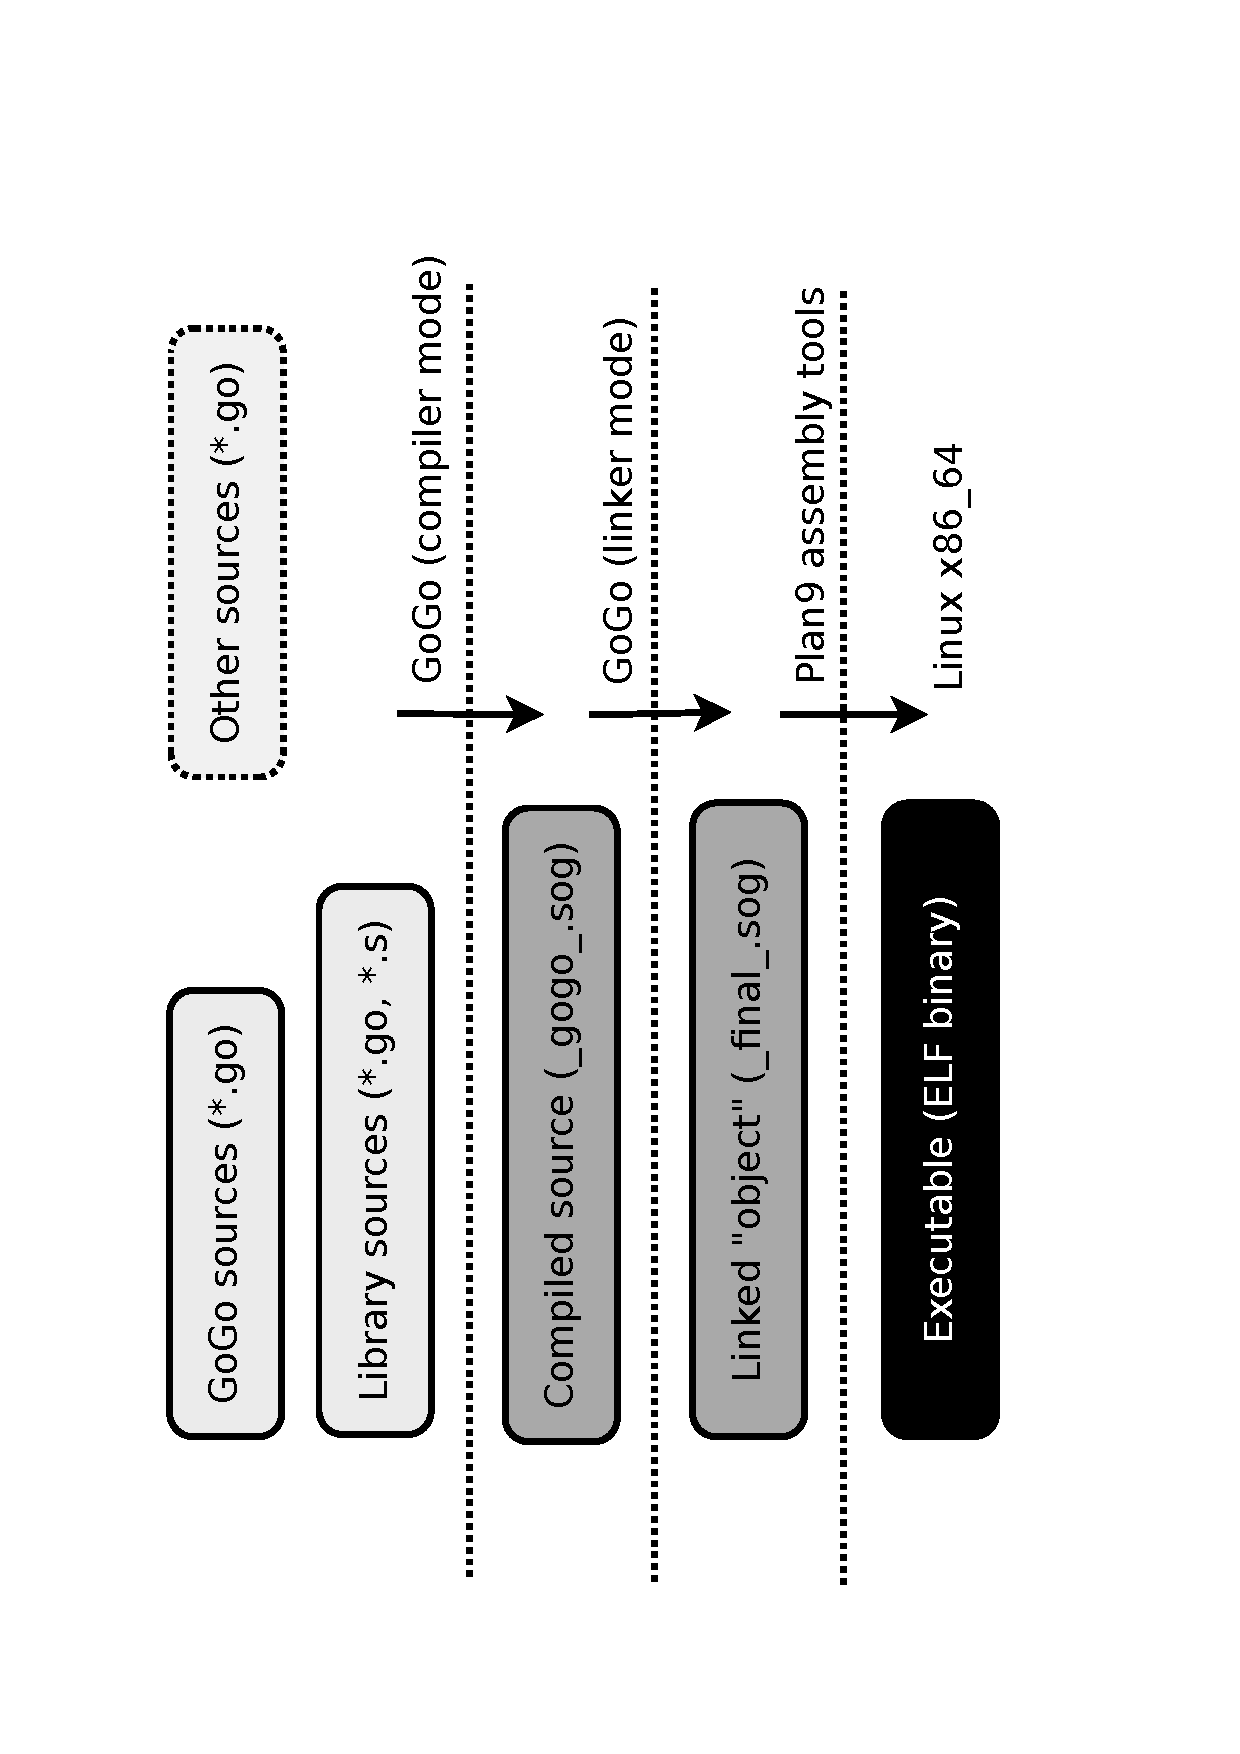
\includegraphics[scale=0.33,angle=-90]{files/building}
    \end{center}
\end{frame}

\frame{\frametitle{Demo}
    \begin{itemize}
        \item Recursive self-compilation
        \item Advanced Fibonacci example
    \end{itemize}
}

\end{document}

